\documentclass[1p]{elsarticle_modified}
%\bibliographystyle{elsarticle-num}

%\usepackage[colorlinks]{hyperref}
%\usepackage{abbrmath_seonhwa} %\Abb, \Ascr, \Acal ,\Abf, \Afrak
\usepackage{amsfonts}
\usepackage{amssymb}
\usepackage{amsmath}
\usepackage{amsthm}
\usepackage{scalefnt}
\usepackage{amsbsy}
\usepackage{kotex}
\usepackage{caption}
\usepackage{subfig}
\usepackage{color}
\usepackage{graphicx}
\usepackage{xcolor} %% white, black, red, green, blue, cyan, magenta, yellow
\usepackage{float}
\usepackage{setspace}
\usepackage{hyperref}

\usepackage{tikz}
\usetikzlibrary{arrows}

\usepackage{multirow}
\usepackage{array} % fixed length table
\usepackage{hhline}

%%%%%%%%%%%%%%%%%%%%%
\makeatletter
\renewcommand*\env@matrix[1][\arraystretch]{%
	\edef\arraystretch{#1}%
	\hskip -\arraycolsep
	\let\@ifnextchar\new@ifnextchar
	\array{*\c@MaxMatrixCols c}}
\makeatother %https://tex.stackexchange.com/questions/14071/how-can-i-increase-the-line-spacing-in-a-matrix
%%%%%%%%%%%%%%%

\usepackage[normalem]{ulem}

\newcommand{\msout}[1]{\ifmmode\text{\sout{\ensuremath{#1}}}\else\sout{#1}\fi}
%SOURCE: \msout is \stkout macro in https://tex.stackexchange.com/questions/20609/strikeout-in-math-mode

\newcommand{\cancel}[1]{
	\ifmmode
	{\color{red}\msout{#1}}
	\else
	{\color{red}\sout{#1}}
	\fi
}

\newcommand{\add}[1]{
	{\color{blue}\uwave{#1}}
}

\newcommand{\replace}[2]{
	\ifmmode
	{\color{red}\msout{#1}}{\color{blue}\uwave{#2}}
	\else
	{\color{red}\sout{#1}}{\color{blue}\uwave{#2}}
	\fi
}

\newcommand{\Sol}{\mathcal{S}} %segment
\newcommand{\D}{D} %diagram
\newcommand{\A}{\mathcal{A}} %arc


%%%%%%%%%%%%%%%%%%%%%%%%%%%%%5 test

\def\sl{\operatorname{\textup{SL}}(2,\Cbb)}
\def\psl{\operatorname{\textup{PSL}}(2,\Cbb)}
\def\quan{\mkern 1mu \triangleright \mkern 1mu}

\theoremstyle{definition}
\newtheorem{thm}{Theorem}[section]
\newtheorem{prop}[thm]{Proposition}
\newtheorem{lem}[thm]{Lemma}
\newtheorem{ques}[thm]{Question}
\newtheorem{cor}[thm]{Corollary}
\newtheorem{defn}[thm]{Definition}
\newtheorem{exam}[thm]{Example}
\newtheorem{rmk}[thm]{Remark}
\newtheorem{alg}[thm]{Algorithm}

\newcommand{\I}{\sqrt{-1}}
\begin{document}

%\begin{frontmatter}
%
%\title{Boundary parabolic representations of knots up to 8 crossings}
%
%%% Group authors per affiliation:
%\author{Yunhi Cho} 
%\address{Department of Mathematics, University of Seoul, Seoul, Korea}
%\ead{yhcho@uos.ac.kr}
%
%
%\author{Seonhwa Kim} %\fnref{s_kim}}
%\address{Center for Geometry and Physics, Institute for Basic Science, Pohang, 37673, Korea}
%\ead{ryeona17@ibs.re.kr}
%
%\author{Hyuk Kim}
%\address{Department of Mathematical Sciences, Seoul National University, Seoul 08826, Korea}
%\ead{hyukkim@snu.ac.kr}
%
%\author{Seokbeom Yoon}
%\address{Department of Mathematical Sciences, Seoul National University, Seoul, 08826,  Korea}
%\ead{sbyoon15@snu.ac.kr}
%
%\begin{abstract}
%We find all boundary parabolic representation of knots up to 8 crossings.
%
%\end{abstract}
%\begin{keyword}
%    \MSC[2010] 57M25 
%\end{keyword}
%
%\end{frontmatter}

%\linenumbers
%\tableofcontents
%
\newcommand\colored[1]{\textcolor{white}{\rule[-0.35ex]{0.8em}{1.4ex}}\kern-0.8em\color{red} #1}%
%\newcommand\colored[1]{\textcolor{white}{ #1}\kern-2.17ex	\textcolor{white}{ #1}\kern-1.81ex	\textcolor{white}{ #1}\kern-2.15ex\color{red}#1	}

{\Large $\underline{12a_{0770}~(K12a_{0770})}$}

\setlength{\tabcolsep}{10pt}
\renewcommand{\arraystretch}{1.6}
\vspace{1cm}\begin{tabular}{m{100pt}>{\centering\arraybackslash}m{274pt}}
\multirow{5}{120pt}{
	\centering
	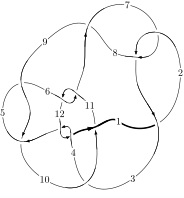
\includegraphics[width=112pt]{../../../GIT/diagram.site/Diagrams/png/1571_12a_0770.png}\\
\ \ \ A knot diagram\footnotemark}&
\allowdisplaybreaks
\textbf{Linearized knot diagam} \\
\cline{2-2}
 &
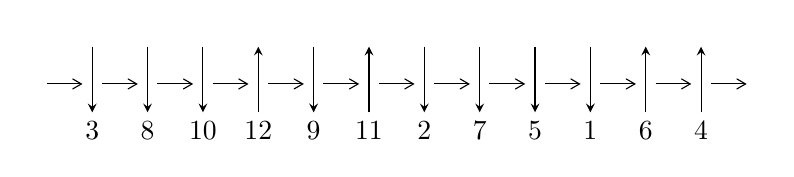
\begin{tikzpicture}[x=20pt, y=17pt]
	% nodes
	\node (C0) at (0, 0) {};
	\node (C1) at (1, 0) {};
	\node (C1U) at (1, +1) {};
	\node (C1D) at (1, -1) {3};

	\node (C2) at (2, 0) {};
	\node (C2U) at (2, +1) {};
	\node (C2D) at (2, -1) {8};

	\node (C3) at (3, 0) {};
	\node (C3U) at (3, +1) {};
	\node (C3D) at (3, -1) {10};

	\node (C4) at (4, 0) {};
	\node (C4U) at (4, +1) {};
	\node (C4D) at (4, -1) {12};

	\node (C5) at (5, 0) {};
	\node (C5U) at (5, +1) {};
	\node (C5D) at (5, -1) {9};

	\node (C6) at (6, 0) {};
	\node (C6U) at (6, +1) {};
	\node (C6D) at (6, -1) {11};

	\node (C7) at (7, 0) {};
	\node (C7U) at (7, +1) {};
	\node (C7D) at (7, -1) {2};

	\node (C8) at (8, 0) {};
	\node (C8U) at (8, +1) {};
	\node (C8D) at (8, -1) {7};

	\node (C9) at (9, 0) {};
	\node (C9U) at (9, +1) {};
	\node (C9D) at (9, -1) {5};

	\node (C10) at (10, 0) {};
	\node (C10U) at (10, +1) {};
	\node (C10D) at (10, -1) {1};

	\node (C11) at (11, 0) {};
	\node (C11U) at (11, +1) {};
	\node (C11D) at (11, -1) {6};

	\node (C12) at (12, 0) {};
	\node (C12U) at (12, +1) {};
	\node (C12D) at (12, -1) {4};
	\node (C13) at (13, 0) {};

	% arrows
	\draw[->,>={angle 60}]
	(C0) edge (C1) (C1) edge (C2) (C2) edge (C3) (C3) edge (C4) (C4) edge (C5) (C5) edge (C6) (C6) edge (C7) (C7) edge (C8) (C8) edge (C9) (C9) edge (C10) (C10) edge (C11) (C11) edge (C12) (C12) edge (C13) ;	\draw[->,>=stealth]
	(C1U) edge (C1D) (C2U) edge (C2D) (C3U) edge (C3D) (C4D) edge (C4U) (C5U) edge (C5D) (C6D) edge (C6U) (C7U) edge (C7D) (C8U) edge (C8D) (C9U) edge (C9D) (C10U) edge (C10D) (C11D) edge (C11U) (C12D) edge (C12U) ;
	\end{tikzpicture} \\
\hhline{~~} \\& 
\textbf{Solving Sequence} \\ \cline{2-2} 
 &
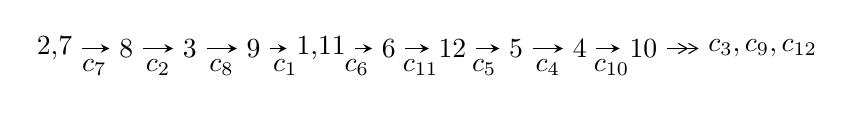
\begin{tikzpicture}[x=23pt, y=7pt]
	% node
	\node (A0) at (-1/8, 0) {2,7};
	\node (A1) at (1, 0) {8};
	\node (A2) at (2, 0) {3};
	\node (A3) at (3, 0) {9};
	\node (A4) at (65/16, 0) {1,11};
	\node (A5) at (41/8, 0) {6};
	\node (A6) at (49/8, 0) {12};
	\node (A7) at (57/8, 0) {5};
	\node (A8) at (65/8, 0) {4};
	\node (A9) at (73/8, 0) {10};
	\node (C1) at (1/2, -1) {$c_{7}$};
	\node (C2) at (3/2, -1) {$c_{2}$};
	\node (C3) at (5/2, -1) {$c_{8}$};
	\node (C4) at (7/2, -1) {$c_{1}$};
	\node (C5) at (37/8, -1) {$c_{6}$};
	\node (C6) at (45/8, -1) {$c_{11}$};
	\node (C7) at (53/8, -1) {$c_{5}$};
	\node (C8) at (61/8, -1) {$c_{4}$};
	\node (C9) at (69/8, -1) {$c_{10}$};
	\node (A10) at (11, 0) {$c_{3},c_{9},c_{12}$};

	% edge
	\draw[->,>=stealth]	
	(A0) edge (A1) (A1) edge (A2) (A2) edge (A3) (A3) edge (A4) (A4) edge (A5) (A5) edge (A6) (A6) edge (A7) (A7) edge (A8) (A8) edge (A9) ;
	\draw[->>,>={angle 60}]	
	(A9) edge (A10);
\end{tikzpicture} \\ 

\end{tabular} \\

\footnotetext{
The image of knot diagram is generated by the software ``\textbf{Draw programme}" developed by Andrew Bartholomew(\url{http://www.layer8.co.uk/maths/draw/index.htm\#Running-draw}), where we modified some parts for our purpose(\url{https://github.com/CATsTAILs/LinksPainter}).
}\phantom \\ \newline 
\centering \textbf{Ideals for irreducible components\footnotemark of $X_{\text{par}}$} 
 
\begin{align*}
I^u_{1}&=\langle 
-6.65043\times10^{180} u^{122}-4.62248\times10^{181} u^{121}+\cdots+5.34068\times10^{181} b+2.74124\times10^{183},\\
\phantom{I^u_{1}}&\phantom{= \langle  }-7.47255\times10^{182} u^{122}-1.31863\times10^{183} u^{121}+\cdots+6.14178\times10^{182} a+1.15546\times10^{184},\\
\phantom{I^u_{1}}&\phantom{= \langle  }u^{123}+u^{122}+\cdots+43 u+23\rangle \\
I^u_{2}&=\langle 
3 u^{21}-3 u^{20}+\cdots+b+2 u,\;-5 u^{21}+7 u^{20}+\cdots+a+2,\;u^{22}-2 u^{21}+\cdots- u+1\rangle \\
I^u_{3}&=\langle 
2 b- a-1,\;a^2+3,\;u+1\rangle \\
\\
\end{align*}
\raggedright * 3 irreducible components of $\dim_{\mathbb{C}}=0$, with total 147 representations.\\
\footnotetext{All coefficients of polynomials are rational numbers. But the coefficients are sometimes approximated in decimal forms when there is not enough margin.}
\newpage
\renewcommand{\arraystretch}{1}
\centering \section*{I. $I^u_{1}= \langle -6.65\times10^{180} u^{122}-4.62\times10^{181} u^{121}+\cdots+5.34\times10^{181} b+2.74\times10^{183},\;-7.47\times10^{182} u^{122}-1.32\times10^{183} u^{121}+\cdots+6.14\times10^{182} a+1.16\times10^{184},\;u^{123}+u^{122}+\cdots+43 u+23 \rangle$}
\flushleft \textbf{(i) Arc colorings}\\
\begin{tabular}{m{7pt} m{180pt} m{7pt} m{180pt} }
\flushright $a_{2}=$&$\begin{pmatrix}0\\u\end{pmatrix}$ \\
\flushright $a_{7}=$&$\begin{pmatrix}1\\0\end{pmatrix}$ \\
\flushright $a_{8}=$&$\begin{pmatrix}1\\u^2\end{pmatrix}$ \\
\flushright $a_{3}=$&$\begin{pmatrix}- u\\- u^3+u\end{pmatrix}$ \\
\flushright $a_{9}=$&$\begin{pmatrix}- u^2+1\\u^2\end{pmatrix}$ \\
\flushright $a_{1}=$&$\begin{pmatrix}u^3\\u^5- u^3+u\end{pmatrix}$ \\
\flushright $a_{11}=$&$\begin{pmatrix}1.21667 u^{122}+2.14697 u^{121}+\cdots-77.9956 u-18.8131\\0.124524 u^{122}+0.865522 u^{121}+\cdots-67.1265 u-51.3275\end{pmatrix}$ \\
\flushright $a_{6}=$&$\begin{pmatrix}-0.0607396 u^{122}+0.475188 u^{121}+\cdots-44.6538 u-69.4270\\1.67317 u^{122}+0.806668 u^{121}+\cdots+5.21204 u+63.7892\end{pmatrix}$ \\
\flushright $a_{12}=$&$\begin{pmatrix}1.23243 u^{122}-0.911083 u^{121}+\cdots+68.7361 u+72.5814\\-2.33691 u^{122}-2.63772 u^{121}+\cdots+131.127 u+1.01620\end{pmatrix}$ \\
\flushright $a_{5}=$&$\begin{pmatrix}0.914222 u^{122}+0.748352 u^{121}+\cdots-27.3667 u-28.7631\\1.49054 u^{122}+0.650958 u^{121}+\cdots+16.0082 u+79.3115\end{pmatrix}$ \\
\flushright $a_{4}=$&$\begin{pmatrix}-1.54515 u^{122}-0.506262 u^{121}+\cdots-7.26446 u-50.9718\\1.79972 u^{122}+0.979358 u^{121}+\cdots-8.27209 u+29.8660\end{pmatrix}$ \\
\flushright $a_{10}=$&$\begin{pmatrix}1.17727 u^{122}+1.92689 u^{121}+\cdots-54.9908 u-7.68351\\-0.328200 u^{122}+0.391498 u^{121}+\cdots-57.6916 u-52.2228\end{pmatrix}$\\&\end{tabular}
\flushleft \textbf{(ii) Obstruction class $= -1$}\\~\\
\flushleft \textbf{(iii) Cusp Shapes $= -1.02390 u^{122}-5.22769 u^{121}+\cdots+262.256 u+134.644$}\\~\\
\newpage\renewcommand{\arraystretch}{1}
\flushleft \textbf{(iv) u-Polynomials at the component}\newline \\
\begin{tabular}{m{50pt}|m{274pt}}
Crossings & \hspace{64pt}u-Polynomials at each crossing \\
\hline $$\begin{aligned}c_{1},c_{8}\end{aligned}$$&$\begin{aligned}
&u^{123}+37 u^{122}+\cdots+8841 u+529
\end{aligned}$\\
\hline $$\begin{aligned}c_{2},c_{7}\end{aligned}$$&$\begin{aligned}
&u^{123}+u^{122}+\cdots+43 u+23
\end{aligned}$\\
\hline $$\begin{aligned}c_{3}\end{aligned}$$&$\begin{aligned}
&u^{123}+u^{122}+\cdots-438 u+319
\end{aligned}$\\
\hline $$\begin{aligned}c_{4},c_{12}\end{aligned}$$&$\begin{aligned}
&u^{123}+5 u^{122}+\cdots+1096 u+193
\end{aligned}$\\
\hline $$\begin{aligned}c_{5},c_{9}\end{aligned}$$&$\begin{aligned}
&u^{123}-3 u^{122}+\cdots-2 u+1
\end{aligned}$\\
\hline $$\begin{aligned}c_{6},c_{11}\end{aligned}$$&$\begin{aligned}
&u^{123}- u^{122}+\cdots-2422 u+317
\end{aligned}$\\
\hline $$\begin{aligned}c_{10}\end{aligned}$$&$\begin{aligned}
&u^{123}-3 u^{122}+\cdots+36 u-1
\end{aligned}$\\
\hline
\end{tabular}\\~\\
\newpage\renewcommand{\arraystretch}{1}
\flushleft \textbf{(v) Riley Polynomials at the component}\newline \\
\begin{tabular}{m{50pt}|m{274pt}}
Crossings & \hspace{64pt}Riley Polynomials at each crossing \\
\hline $$\begin{aligned}c_{1},c_{8}\end{aligned}$$&$\begin{aligned}
&y^{123}+107 y^{122}+\cdots-3332343 y-279841
\end{aligned}$\\
\hline $$\begin{aligned}c_{2},c_{7}\end{aligned}$$&$\begin{aligned}
&y^{123}-37 y^{122}+\cdots+8841 y-529
\end{aligned}$\\
\hline $$\begin{aligned}c_{3}\end{aligned}$$&$\begin{aligned}
&y^{123}+23 y^{122}+\cdots-8257190 y-101761
\end{aligned}$\\
\hline $$\begin{aligned}c_{4},c_{12}\end{aligned}$$&$\begin{aligned}
&y^{123}+87 y^{122}+\cdots-679762 y-37249
\end{aligned}$\\
\hline $$\begin{aligned}c_{5},c_{9}\end{aligned}$$&$\begin{aligned}
&y^{123}+77 y^{122}+\cdots-114 y-1
\end{aligned}$\\
\hline $$\begin{aligned}c_{6},c_{11}\end{aligned}$$&$\begin{aligned}
&y^{123}+75 y^{122}+\cdots+1511772 y-100489
\end{aligned}$\\
\hline $$\begin{aligned}c_{10}\end{aligned}$$&$\begin{aligned}
&y^{123}-7 y^{122}+\cdots-146 y-1
\end{aligned}$\\
\hline
\end{tabular}\\~\\
\newpage\flushleft \textbf{(vi) Complex Volumes and Cusp Shapes}
$$\begin{array}{c|c|c}  
\text{Solutions to }I^u_{1}& \I (\text{vol} + \sqrt{-1}CS) & \text{Cusp shape}\\
 \hline 
\begin{aligned}
u &= \phantom{-}0.998038 + 0.111520 I \\
a &= -0.618593 - 1.235120 I \\
b &= \phantom{-}0.464560 - 0.829256 I\end{aligned}
 & -3.64634 - 2.82809 I & \phantom{-0.000000 } 0 \\ \hline\begin{aligned}
u &= \phantom{-}0.998038 - 0.111520 I \\
a &= -0.618593 + 1.235120 I \\
b &= \phantom{-}0.464560 + 0.829256 I\end{aligned}
 & -3.64634 + 2.82809 I & \phantom{-0.000000 } 0 \\ \hline\begin{aligned}
u &= -1.008390 + 0.041848 I \\
a &= -0.012986 + 1.238690 I \\
b &= \phantom{-}0.74198 + 1.33457 I\end{aligned}
 & -5.23839 + 3.65926 I & \phantom{-0.000000 } 0 \\ \hline\begin{aligned}
u &= -1.008390 - 0.041848 I \\
a &= -0.012986 - 1.238690 I \\
b &= \phantom{-}0.74198 - 1.33457 I\end{aligned}
 & -5.23839 - 3.65926 I & \phantom{-0.000000 } 0 \\ \hline\begin{aligned}
u &= \phantom{-}0.747677 + 0.678061 I \\
a &= \phantom{-}1.29904 + 1.42318 I \\
b &= -1.10040 - 1.00468 I\end{aligned}
 & -0.28697 + 3.57568 I & \phantom{-0.000000 } 0 \\ \hline\begin{aligned}
u &= \phantom{-}0.747677 - 0.678061 I \\
a &= \phantom{-}1.29904 - 1.42318 I \\
b &= -1.10040 + 1.00468 I\end{aligned}
 & -0.28697 - 3.57568 I & \phantom{-0.000000 } 0 \\ \hline\begin{aligned}
u &= \phantom{-}0.978634 + 0.099967 I \\
a &= -0.575223 - 1.000370 I \\
b &= \phantom{-}0.532319 - 0.539416 I\end{aligned}
 & -3.62329 - 2.84767 I & \phantom{-0.000000 } 0 \\ \hline\begin{aligned}
u &= \phantom{-}0.978634 - 0.099967 I \\
a &= -0.575223 + 1.000370 I \\
b &= \phantom{-}0.532319 + 0.539416 I\end{aligned}
 & -3.62329 + 2.84767 I & \phantom{-0.000000 } 0 \\ \hline\begin{aligned}
u &= \phantom{-}0.999685 + 0.318338 I \\
a &= \phantom{-}0.846148 + 0.812960 I \\
b &= \phantom{-}0.02291 + 1.41918 I\end{aligned}
 & -8.44641 - 0.32156 I & \phantom{-0.000000 } 0 \\ \hline\begin{aligned}
u &= \phantom{-}0.999685 - 0.318338 I \\
a &= \phantom{-}0.846148 - 0.812960 I \\
b &= \phantom{-}0.02291 - 1.41918 I\end{aligned}
 & -8.44641 + 0.32156 I & \phantom{-0.000000 } 0\\
 \hline 
 \end{array}$$\newpage$$\begin{array}{c|c|c}  
\text{Solutions to }I^u_{1}& \I (\text{vol} + \sqrt{-1}CS) & \text{Cusp shape}\\
 \hline 
\begin{aligned}
u &= \phantom{-}0.694646 + 0.643454 I \\
a &= \phantom{-}0.846743 - 0.636508 I \\
b &= -0.163630 - 0.059486 I\end{aligned}
 & \phantom{-}2.48058 - 1.47346 I & \phantom{-0.000000 } 0 \\ \hline\begin{aligned}
u &= \phantom{-}0.694646 - 0.643454 I \\
a &= \phantom{-}0.846743 + 0.636508 I \\
b &= -0.163630 + 0.059486 I\end{aligned}
 & \phantom{-}2.48058 + 1.47346 I & \phantom{-0.000000 } 0 \\ \hline\begin{aligned}
u &= -0.718678 + 0.775205 I \\
a &= \phantom{-}1.45433 - 0.51245 I \\
b &= -0.796471 + 0.555784 I\end{aligned}
 & \phantom{-}2.25372 - 2.40345 I & \phantom{-0.000000 } 0 \\ \hline\begin{aligned}
u &= -0.718678 - 0.775205 I \\
a &= \phantom{-}1.45433 + 0.51245 I \\
b &= -0.796471 - 0.555784 I\end{aligned}
 & \phantom{-}2.25372 + 2.40345 I & \phantom{-0.000000 } 0 \\ \hline\begin{aligned}
u &= -0.828714 + 0.440216 I \\
a &= \phantom{-}0.405860 + 0.873938 I \\
b &= \phantom{-}0.530574 - 0.657586 I\end{aligned}
 & -1.69210 + 2.01686 I & \phantom{-0.000000 } 0 \\ \hline\begin{aligned}
u &= -0.828714 - 0.440216 I \\
a &= \phantom{-}0.405860 - 0.873938 I \\
b &= \phantom{-}0.530574 + 0.657586 I\end{aligned}
 & -1.69210 - 2.01686 I & \phantom{-0.000000 } 0 \\ \hline\begin{aligned}
u &= -0.903346 + 0.243331 I \\
a &= \phantom{-}0.0407501 - 0.0294218 I \\
b &= -1.183180 - 0.102475 I\end{aligned}
 & -1.43303 + 6.80135 I & \phantom{-0.000000 } 0 \\ \hline\begin{aligned}
u &= -0.903346 - 0.243331 I \\
a &= \phantom{-}0.0407501 + 0.0294218 I \\
b &= -1.183180 + 0.102475 I\end{aligned}
 & -1.43303 - 6.80135 I & \phantom{-0.000000 } 0 \\ \hline\begin{aligned}
u &= \phantom{-}1.062020 + 0.073185 I \\
a &= -0.736389 - 1.157230 I \\
b &= \phantom{-}0.097415 - 0.752583 I\end{aligned}
 & -3.59485 - 2.77429 I & \phantom{-0.000000 } 0 \\ \hline\begin{aligned}
u &= \phantom{-}1.062020 - 0.073185 I \\
a &= -0.736389 + 1.157230 I \\
b &= \phantom{-}0.097415 + 0.752583 I\end{aligned}
 & -3.59485 + 2.77429 I & \phantom{-0.000000 } 0\\
 \hline 
 \end{array}$$\newpage$$\begin{array}{c|c|c}  
\text{Solutions to }I^u_{1}& \I (\text{vol} + \sqrt{-1}CS) & \text{Cusp shape}\\
 \hline 
\begin{aligned}
u &= -0.771064 + 0.741605 I \\
a &= -0.110952 + 1.386560 I \\
b &= \phantom{-}0.516847 - 1.169790 I\end{aligned}
 & -1.99581 + 1.48737 I & \phantom{-0.000000 } 0 \\ \hline\begin{aligned}
u &= -0.771064 - 0.741605 I \\
a &= -0.110952 - 1.386560 I \\
b &= \phantom{-}0.516847 + 1.169790 I\end{aligned}
 & -1.99581 - 1.48737 I & \phantom{-0.000000 } 0 \\ \hline\begin{aligned}
u &= -1.040000 + 0.262995 I \\
a &= -1.40149 + 0.98571 I \\
b &= \phantom{-}0.264976 + 1.307830 I\end{aligned}
 & -8.72461 + 5.99285 I & \phantom{-0.000000 } 0 \\ \hline\begin{aligned}
u &= -1.040000 - 0.262995 I \\
a &= -1.40149 - 0.98571 I \\
b &= \phantom{-}0.264976 - 1.307830 I\end{aligned}
 & -8.72461 - 5.99285 I & \phantom{-0.000000 } 0 \\ \hline\begin{aligned}
u &= -0.897567 + 0.593044 I \\
a &= \phantom{-}0.702479 - 0.017392 I \\
b &= \phantom{-}0.139182 - 0.979590 I\end{aligned}
 & -1.12457 + 2.29817 I & \phantom{-0.000000 } 0 \\ \hline\begin{aligned}
u &= -0.897567 - 0.593044 I \\
a &= \phantom{-}0.702479 + 0.017392 I \\
b &= \phantom{-}0.139182 + 0.979590 I\end{aligned}
 & -1.12457 - 2.29817 I & \phantom{-0.000000 } 0 \\ \hline\begin{aligned}
u &= \phantom{-}0.245012 + 0.890518 I \\
a &= -0.355572 + 0.069784 I \\
b &= \phantom{-}0.419312 - 0.758001 I\end{aligned}
 & \phantom{-}3.31588 - 1.85610 I & \phantom{-0.000000 } 0 \\ \hline\begin{aligned}
u &= \phantom{-}0.245012 - 0.890518 I \\
a &= -0.355572 - 0.069784 I \\
b &= \phantom{-}0.419312 + 0.758001 I\end{aligned}
 & \phantom{-}3.31588 + 1.85610 I & \phantom{-0.000000 } 0 \\ \hline\begin{aligned}
u &= \phantom{-}0.819637 + 0.401676 I \\
a &= \phantom{-}0.261319 - 0.494561 I \\
b &= -0.539925 + 0.154824 I\end{aligned}
 & \phantom{-}1.67415 - 2.68529 I & \phantom{-0.000000 } 0 \\ \hline\begin{aligned}
u &= \phantom{-}0.819637 - 0.401676 I \\
a &= \phantom{-}0.261319 + 0.494561 I \\
b &= -0.539925 - 0.154824 I\end{aligned}
 & \phantom{-}1.67415 + 2.68529 I & \phantom{-0.000000 } 0\\
 \hline 
 \end{array}$$\newpage$$\begin{array}{c|c|c}  
\text{Solutions to }I^u_{1}& \I (\text{vol} + \sqrt{-1}CS) & \text{Cusp shape}\\
 \hline 
\begin{aligned}
u &= -0.832068 + 0.700606 I \\
a &= \phantom{-}2.25867 - 0.20449 I \\
b &= -0.161300 - 0.591037 I\end{aligned}
 & \phantom{-}0.85788 - 2.20310 I & \phantom{-0.000000 } 0 \\ \hline\begin{aligned}
u &= -0.832068 - 0.700606 I \\
a &= \phantom{-}2.25867 + 0.20449 I \\
b &= -0.161300 + 0.591037 I\end{aligned}
 & \phantom{-}0.85788 + 2.20310 I & \phantom{-0.000000 } 0 \\ \hline\begin{aligned}
u &= -0.745115 + 0.794136 I \\
a &= \phantom{-}1.107990 - 0.745099 I \\
b &= -0.633546 + 0.858719 I\end{aligned}
 & \phantom{-}2.45030 - 2.24805 I & \phantom{-0.000000 } 0 \\ \hline\begin{aligned}
u &= -0.745115 - 0.794136 I \\
a &= \phantom{-}1.107990 + 0.745099 I \\
b &= -0.633546 - 0.858719 I\end{aligned}
 & \phantom{-}2.45030 + 2.24805 I & \phantom{-0.000000 } 0 \\ \hline\begin{aligned}
u &= -0.586117 + 0.921962 I \\
a &= -0.124249 + 0.255359 I \\
b &= \phantom{-}0.423531 - 1.046930 I\end{aligned}
 & \phantom{-}2.31520 + 1.08669 I & \phantom{-0.000000 } 0 \\ \hline\begin{aligned}
u &= -0.586117 - 0.921962 I \\
a &= -0.124249 - 0.255359 I \\
b &= \phantom{-}0.423531 + 1.046930 I\end{aligned}
 & \phantom{-}2.31520 - 1.08669 I & \phantom{-0.000000 } 0 \\ \hline\begin{aligned}
u &= -0.038136 + 0.876287 I \\
a &= -0.551055 - 0.730714 I \\
b &= \phantom{-}0.513871 + 1.117790 I\end{aligned}
 & -1.63003 + 8.62110 I & \phantom{-0.000000 } 0 \\ \hline\begin{aligned}
u &= -0.038136 - 0.876287 I \\
a &= -0.551055 + 0.730714 I \\
b &= \phantom{-}0.513871 - 1.117790 I\end{aligned}
 & -1.63003 - 8.62110 I & \phantom{-0.000000 } 0 \\ \hline\begin{aligned}
u &= \phantom{-}0.862609 + 0.722091 I \\
a &= \phantom{-}1.95306 - 0.13787 I \\
b &= -0.454401 + 0.739122 I\end{aligned}
 & \phantom{-}2.80440 - 2.13090 I & \phantom{-0.000000 } 0 \\ \hline\begin{aligned}
u &= \phantom{-}0.862609 - 0.722091 I \\
a &= \phantom{-}1.95306 + 0.13787 I \\
b &= -0.454401 - 0.739122 I\end{aligned}
 & \phantom{-}2.80440 + 2.13090 I & \phantom{-0.000000 } 0\\
 \hline 
 \end{array}$$\newpage$$\begin{array}{c|c|c}  
\text{Solutions to }I^u_{1}& \I (\text{vol} + \sqrt{-1}CS) & \text{Cusp shape}\\
 \hline 
\begin{aligned}
u &= \phantom{-}0.961243 + 0.587894 I \\
a &= \phantom{-}1.14619 - 0.86535 I \\
b &= \phantom{-}0.31694 + 1.38447 I\end{aligned}
 & -2.03643 - 1.93180 I & \phantom{-0.000000 } 0 \\ \hline\begin{aligned}
u &= \phantom{-}0.961243 - 0.587894 I \\
a &= \phantom{-}1.14619 + 0.86535 I \\
b &= \phantom{-}0.31694 - 1.38447 I\end{aligned}
 & -2.03643 + 1.93180 I & \phantom{-0.000000 } 0 \\ \hline\begin{aligned}
u &= -0.873179 + 0.719044 I \\
a &= -1.56461 - 1.14251 I \\
b &= -0.05346 + 2.18005 I\end{aligned}
 & -3.82458 + 2.74777 I & \phantom{-0.000000 } 0 \\ \hline\begin{aligned}
u &= -0.873179 - 0.719044 I \\
a &= -1.56461 + 1.14251 I \\
b &= -0.05346 - 2.18005 I\end{aligned}
 & -3.82458 - 2.74777 I & \phantom{-0.000000 } 0 \\ \hline\begin{aligned}
u &= -0.826141 + 0.781445 I \\
a &= \phantom{-}1.070400 - 0.503843 I \\
b &= -0.612674 + 1.078900 I\end{aligned}
 & \phantom{-}3.46834 - 2.97155 I & \phantom{-0.000000 } 0 \\ \hline\begin{aligned}
u &= -0.826141 - 0.781445 I \\
a &= \phantom{-}1.070400 + 0.503843 I \\
b &= -0.612674 - 1.078900 I\end{aligned}
 & \phantom{-}3.46834 + 2.97155 I & \phantom{-0.000000 } 0 \\ \hline\begin{aligned}
u &= \phantom{-}0.852358 + 0.753126 I \\
a &= \phantom{-}0.237441 + 0.203080 I \\
b &= -0.436051 - 1.275240 I\end{aligned}
 & \phantom{-}3.86620 - 1.44750 I & \phantom{-0.000000 } 0 \\ \hline\begin{aligned}
u &= \phantom{-}0.852358 - 0.753126 I \\
a &= \phantom{-}0.237441 - 0.203080 I \\
b &= -0.436051 + 1.275240 I\end{aligned}
 & \phantom{-}3.86620 + 1.44750 I & \phantom{-0.000000 } 0 \\ \hline\begin{aligned}
u &= \phantom{-}0.787621 + 0.829507 I \\
a &= -1.87946 - 0.52483 I \\
b &= \phantom{-}1.41777 - 0.40004 I\end{aligned}
 & \phantom{-}5.34270 + 5.05268 I & \phantom{-0.000000 } 0 \\ \hline\begin{aligned}
u &= \phantom{-}0.787621 - 0.829507 I \\
a &= -1.87946 + 0.52483 I \\
b &= \phantom{-}1.41777 + 0.40004 I\end{aligned}
 & \phantom{-}5.34270 - 5.05268 I & \phantom{-0.000000 } 0\\
 \hline 
 \end{array}$$\newpage$$\begin{array}{c|c|c}  
\text{Solutions to }I^u_{1}& \I (\text{vol} + \sqrt{-1}CS) & \text{Cusp shape}\\
 \hline 
\begin{aligned}
u &= \phantom{-}0.887733 + 0.721472 I \\
a &= -0.856295 - 0.891714 I \\
b &= \phantom{-}0.560141 + 0.584146 I\end{aligned}
 & \phantom{-}2.72547 - 3.38209 I & \phantom{-0.000000 } 0 \\ \hline\begin{aligned}
u &= \phantom{-}0.887733 - 0.721472 I \\
a &= -0.856295 + 0.891714 I \\
b &= \phantom{-}0.560141 - 0.584146 I\end{aligned}
 & \phantom{-}2.72547 + 3.38209 I & \phantom{-0.000000 } 0 \\ \hline\begin{aligned}
u &= \phantom{-}0.758416 + 0.865706 I \\
a &= \phantom{-}0.804802 + 1.078350 I \\
b &= -0.408380 - 1.099450 I\end{aligned}
 & -1.26568 + 5.11585 I & \phantom{-0.000000 } 0 \\ \hline\begin{aligned}
u &= \phantom{-}0.758416 - 0.865706 I \\
a &= \phantom{-}0.804802 - 1.078350 I \\
b &= -0.408380 + 1.099450 I\end{aligned}
 & -1.26568 - 5.11585 I & \phantom{-0.000000 } 0 \\ \hline\begin{aligned}
u &= -0.916667 + 0.696677 I \\
a &= -1.39838 + 0.44542 I \\
b &= \phantom{-}0.295926 - 0.386739 I\end{aligned}
 & \phantom{-}0.58974 + 7.57307 I & \phantom{-0.000000 } 0 \\ \hline\begin{aligned}
u &= -0.916667 - 0.696677 I \\
a &= -1.39838 - 0.44542 I \\
b &= \phantom{-}0.295926 + 0.386739 I\end{aligned}
 & \phantom{-}0.58974 - 7.57307 I & \phantom{-0.000000 } 0 \\ \hline\begin{aligned}
u &= \phantom{-}0.706014 + 0.915678 I \\
a &= -0.624192 - 0.687267 I \\
b &= \phantom{-}0.657698 + 1.214410 I\end{aligned}
 & \phantom{-}6.59960 + 6.11951 I & \phantom{-0.000000 } 0 \\ \hline\begin{aligned}
u &= \phantom{-}0.706014 - 0.915678 I \\
a &= -0.624192 + 0.687267 I \\
b &= \phantom{-}0.657698 - 1.214410 I\end{aligned}
 & \phantom{-}6.59960 - 6.11951 I & \phantom{-0.000000 } 0 \\ \hline\begin{aligned}
u &= -0.718343 + 0.910366 I \\
a &= -0.807984 + 0.965034 I \\
b &= \phantom{-}0.75916 - 1.30609 I\end{aligned}
 & \phantom{-}2.36046 - 12.44930 I & \phantom{-0.000000 } 0 \\ \hline\begin{aligned}
u &= -0.718343 - 0.910366 I \\
a &= -0.807984 - 0.965034 I \\
b &= \phantom{-}0.75916 + 1.30609 I\end{aligned}
 & \phantom{-}2.36046 + 12.44930 I & \phantom{-0.000000 } 0\\
 \hline 
 \end{array}$$\newpage$$\begin{array}{c|c|c}  
\text{Solutions to }I^u_{1}& \I (\text{vol} + \sqrt{-1}CS) & \text{Cusp shape}\\
 \hline 
\begin{aligned}
u &= \phantom{-}0.900961 + 0.743227 I \\
a &= -1.75793 - 0.52878 I \\
b &= \phantom{-}0.343286 - 1.313990 I\end{aligned}
 & \phantom{-}3.71549 - 4.22857 I & \phantom{-0.000000 } 0 \\ \hline\begin{aligned}
u &= \phantom{-}0.900961 - 0.743227 I \\
a &= -1.75793 + 0.52878 I \\
b &= \phantom{-}0.343286 + 1.313990 I\end{aligned}
 & \phantom{-}3.71549 + 4.22857 I & \phantom{-0.000000 } 0 \\ \hline\begin{aligned}
u &= \phantom{-}1.140660 + 0.278300 I \\
a &= \phantom{-}0.737848 + 1.093620 I \\
b &= -0.538495 + 1.302820 I\end{aligned}
 & -5.67717 - 12.45260 I & \phantom{-0.000000 } 0 \\ \hline\begin{aligned}
u &= \phantom{-}1.140660 - 0.278300 I \\
a &= \phantom{-}0.737848 - 1.093620 I \\
b &= -0.538495 - 1.302820 I\end{aligned}
 & -5.67717 + 12.45260 I & \phantom{-0.000000 } 0 \\ \hline\begin{aligned}
u &= \phantom{-}0.813009 + 0.120512 I \\
a &= -0.23268 - 3.53099 I \\
b &= \phantom{-}0.315947 - 0.920401 I\end{aligned}
 & -2.01877 - 5.28852 I & \phantom{-0.000000 } 0 \\ \hline\begin{aligned}
u &= \phantom{-}0.813009 - 0.120512 I \\
a &= -0.23268 + 3.53099 I \\
b &= \phantom{-}0.315947 + 0.920401 I\end{aligned}
 & -2.01877 + 5.28852 I & \phantom{-0.000000 } 0 \\ \hline\begin{aligned}
u &= \phantom{-}0.960387 + 0.682857 I \\
a &= -2.48484 - 0.60816 I \\
b &= \phantom{-}1.10630 - 1.19956 I\end{aligned}
 & -0.94330 - 8.86692 I & \phantom{-0.000000 } 0 \\ \hline\begin{aligned}
u &= \phantom{-}0.960387 - 0.682857 I \\
a &= -2.48484 + 0.60816 I \\
b &= \phantom{-}1.10630 + 1.19956 I\end{aligned}
 & -0.94330 + 8.86692 I & \phantom{-0.000000 } 0 \\ \hline\begin{aligned}
u &= -0.813819 + 0.859589 I \\
a &= -1.336780 + 0.401490 I \\
b &= \phantom{-}1.039350 + 0.325117 I\end{aligned}
 & \phantom{-}9.35496 - 0.04602 I & \phantom{-0.000000 } 0 \\ \hline\begin{aligned}
u &= -0.813819 - 0.859589 I \\
a &= -1.336780 - 0.401490 I \\
b &= \phantom{-}1.039350 - 0.325117 I\end{aligned}
 & \phantom{-}9.35496 + 0.04602 I & \phantom{-0.000000 } 0\\
 \hline 
 \end{array}$$\newpage$$\begin{array}{c|c|c}  
\text{Solutions to }I^u_{1}& \I (\text{vol} + \sqrt{-1}CS) & \text{Cusp shape}\\
 \hline 
\begin{aligned}
u &= -0.936883 + 0.724277 I \\
a &= \phantom{-}1.98061 + 0.39240 I \\
b &= -0.59881 - 1.36704 I\end{aligned}
 & -2.47707 + 4.09068 I & \phantom{-0.000000 } 0 \\ \hline\begin{aligned}
u &= -0.936883 - 0.724277 I \\
a &= \phantom{-}1.98061 - 0.39240 I \\
b &= -0.59881 + 1.36704 I\end{aligned}
 & -2.47707 - 4.09068 I & \phantom{-0.000000 } 0 \\ \hline\begin{aligned}
u &= -0.809882\phantom{ +0.000000I} \\
a &= -0.230136\phantom{ +0.000000I} \\
b &= \phantom{-}0.468179\phantom{ +0.000000I}\end{aligned}
 & -1.31525\phantom{ +0.000000I} & -6.85520\phantom{ +0.000000I} \\ \hline\begin{aligned}
u &= -0.928238 + 0.754910 I \\
a &= -2.30996 + 0.61386 I \\
b &= \phantom{-}0.557724 + 1.130270 I\end{aligned}
 & \phantom{-}3.15268 + 8.76794 I & \phantom{-0.000000 } 0 \\ \hline\begin{aligned}
u &= -0.928238 - 0.754910 I \\
a &= -2.30996 - 0.61386 I \\
b &= \phantom{-}0.557724 - 1.130270 I\end{aligned}
 & \phantom{-}3.15268 - 8.76794 I & \phantom{-0.000000 } 0 \\ \hline\begin{aligned}
u &= -0.798815 + 0.045097 I \\
a &= \phantom{-}1.24092 + 2.64289 I \\
b &= \phantom{-}0.059987 + 1.041400 I\end{aligned}
 & -0.780386 + 0.986928 I & -7.33577 + 0. I\phantom{ +0.000000I} \\ \hline\begin{aligned}
u &= -0.798815 - 0.045097 I \\
a &= \phantom{-}1.24092 - 2.64289 I \\
b &= \phantom{-}0.059987 - 1.041400 I\end{aligned}
 & -0.780386 - 0.986928 I & -7.33577 + 0. I\phantom{ +0.000000I} \\ \hline\begin{aligned}
u &= \phantom{-}0.796042 + 0.076675 I \\
a &= \phantom{-}1.01452 + 1.61059 I \\
b &= -0.22148 + 1.83294 I\end{aligned}
 & -7.40333 - 0.39146 I & -12.24132 - 5.59979 I \\ \hline\begin{aligned}
u &= \phantom{-}0.796042 - 0.076675 I \\
a &= \phantom{-}1.01452 - 1.61059 I \\
b &= -0.22148 - 1.83294 I\end{aligned}
 & -7.40333 + 0.39146 I & -12.24132 + 5.59979 I \\ \hline\begin{aligned}
u &= -0.987452 + 0.715297 I \\
a &= -1.94054 + 0.76734 I \\
b &= \phantom{-}0.827683 + 0.651069 I\end{aligned}
 & \phantom{-}1.43912 + 8.05022 I & \phantom{-0.000000 } 0\\
 \hline 
 \end{array}$$\newpage$$\begin{array}{c|c|c}  
\text{Solutions to }I^u_{1}& \I (\text{vol} + \sqrt{-1}CS) & \text{Cusp shape}\\
 \hline 
\begin{aligned}
u &= -0.987452 - 0.715297 I \\
a &= -1.94054 - 0.76734 I \\
b &= \phantom{-}0.827683 - 0.651069 I\end{aligned}
 & \phantom{-}1.43912 - 8.05022 I & \phantom{-0.000000 } 0 \\ \hline\begin{aligned}
u &= -1.185750 + 0.293560 I \\
a &= -0.746021 + 0.436699 I \\
b &= -0.298245 + 1.105680 I\end{aligned}
 & -5.59178 - 4.46851 I & \phantom{-0.000000 } 0 \\ \hline\begin{aligned}
u &= -1.185750 - 0.293560 I \\
a &= -0.746021 - 0.436699 I \\
b &= -0.298245 - 1.105680 I\end{aligned}
 & -5.59178 + 4.46851 I & \phantom{-0.000000 } 0 \\ \hline\begin{aligned}
u &= \phantom{-}0.482789 + 0.609312 I \\
a &= \phantom{-}1.11654 - 1.27200 I \\
b &= -0.432805 + 1.108760 I\end{aligned}
 & -0.75905 - 2.63678 I & -4.00000 + 3.70377 I \\ \hline\begin{aligned}
u &= \phantom{-}0.482789 - 0.609312 I \\
a &= \phantom{-}1.11654 + 1.27200 I \\
b &= -0.432805 - 1.108760 I\end{aligned}
 & -0.75905 + 2.63678 I & -4.00000 - 3.70377 I \\ \hline\begin{aligned}
u &= \phantom{-}0.892271 + 0.839255 I \\
a &= -0.601178 - 1.069560 I \\
b &= \phantom{-}0.650357 + 0.349315 I\end{aligned}
 & \phantom{-}5.44982 - 3.99818 I & \phantom{-0.000000 } 0 \\ \hline\begin{aligned}
u &= \phantom{-}0.892271 - 0.839255 I \\
a &= -0.601178 + 1.069560 I \\
b &= \phantom{-}0.650357 - 0.349315 I\end{aligned}
 & \phantom{-}5.44982 + 3.99818 I & \phantom{-0.000000 } 0 \\ \hline\begin{aligned}
u &= \phantom{-}0.909301 + 0.820936 I \\
a &= \phantom{-}1.258640 - 0.210367 I \\
b &= -0.742377 + 0.414370 I\end{aligned}
 & \phantom{-}5.38340 - 2.18763 I & \phantom{-0.000000 } 0 \\ \hline\begin{aligned}
u &= \phantom{-}0.909301 - 0.820936 I \\
a &= \phantom{-}1.258640 + 0.210367 I \\
b &= -0.742377 - 0.414370 I\end{aligned}
 & \phantom{-}5.38340 + 2.18763 I & \phantom{-0.000000 } 0 \\ \hline\begin{aligned}
u &= -0.986250 + 0.736928 I \\
a &= -2.03098 + 0.35816 I \\
b &= \phantom{-}0.618675 + 0.939690 I\end{aligned}
 & \phantom{-}1.71455 + 8.02792 I & \phantom{-0.000000 } 0\\
 \hline 
 \end{array}$$\newpage$$\begin{array}{c|c|c}  
\text{Solutions to }I^u_{1}& \I (\text{vol} + \sqrt{-1}CS) & \text{Cusp shape}\\
 \hline 
\begin{aligned}
u &= -0.986250 - 0.736928 I \\
a &= -2.03098 - 0.35816 I \\
b &= \phantom{-}0.618675 - 0.939690 I\end{aligned}
 & \phantom{-}1.71455 - 8.02792 I & \phantom{-0.000000 } 0 \\ \hline\begin{aligned}
u &= -1.203380 + 0.286854 I \\
a &= \phantom{-}0.480013 - 0.986726 I \\
b &= -0.367702 - 1.128060 I\end{aligned}
 & -1.56465 + 5.76869 I & \phantom{-0.000000 } 0 \\ \hline\begin{aligned}
u &= -1.203380 - 0.286854 I \\
a &= \phantom{-}0.480013 + 0.986726 I \\
b &= -0.367702 + 1.128060 I\end{aligned}
 & -1.56465 - 5.76869 I & \phantom{-0.000000 } 0 \\ \hline\begin{aligned}
u &= \phantom{-}0.971042 + 0.769166 I \\
a &= \phantom{-}1.20489 + 1.25291 I \\
b &= -1.50331 - 0.31741 I\end{aligned}
 & \phantom{-}4.77387 - 11.03380 I & \phantom{-0.000000 } 0 \\ \hline\begin{aligned}
u &= \phantom{-}0.971042 - 0.769166 I \\
a &= \phantom{-}1.20489 - 1.25291 I \\
b &= -1.50331 + 0.31741 I\end{aligned}
 & \phantom{-}4.77387 + 11.03380 I & \phantom{-0.000000 } 0 \\ \hline\begin{aligned}
u &= -0.967816 + 0.798846 I \\
a &= \phantom{-}0.910943 - 0.780219 I \\
b &= -1.080580 + 0.221639 I\end{aligned}
 & \phantom{-}8.87149 + 6.21107 I & \phantom{-0.000000 } 0 \\ \hline\begin{aligned}
u &= -0.967816 - 0.798846 I \\
a &= \phantom{-}0.910943 + 0.780219 I \\
b &= -1.080580 - 0.221639 I\end{aligned}
 & \phantom{-}8.87149 - 6.21107 I & \phantom{-0.000000 } 0 \\ \hline\begin{aligned}
u &= -0.914060 + 0.864103 I \\
a &= \phantom{-}0.496423 + 1.220680 I \\
b &= -0.032726 - 0.721159 I\end{aligned}
 & \phantom{-}6.99072 + 3.20060 I & \phantom{-0.000000 } 0 \\ \hline\begin{aligned}
u &= -0.914060 - 0.864103 I \\
a &= \phantom{-}0.496423 - 1.220680 I \\
b &= -0.032726 + 0.721159 I\end{aligned}
 & \phantom{-}6.99072 - 3.20060 I & \phantom{-0.000000 } 0 \\ \hline\begin{aligned}
u &= \phantom{-}1.004730 + 0.776456 I \\
a &= -2.08514 + 0.19800 I \\
b &= \phantom{-}0.461508 - 1.149300 I\end{aligned}
 & -2.03159 - 11.22630 I & \phantom{-0.000000 } 0\\
 \hline 
 \end{array}$$\newpage$$\begin{array}{c|c|c}  
\text{Solutions to }I^u_{1}& \I (\text{vol} + \sqrt{-1}CS) & \text{Cusp shape}\\
 \hline 
\begin{aligned}
u &= \phantom{-}1.004730 - 0.776456 I \\
a &= -2.08514 - 0.19800 I \\
b &= \phantom{-}0.461508 + 1.149300 I\end{aligned}
 & -2.03159 + 11.22630 I & \phantom{-0.000000 } 0 \\ \hline\begin{aligned}
u &= \phantom{-}1.084670 + 0.665154 I \\
a &= -0.963426 - 0.321344 I \\
b &= \phantom{-}0.016691 - 0.674808 I\end{aligned}
 & \phantom{-}1.06519 - 3.48213 I & \phantom{-0.000000 } 0 \\ \hline\begin{aligned}
u &= \phantom{-}1.084670 - 0.665154 I \\
a &= -0.963426 + 0.321344 I \\
b &= \phantom{-}0.016691 + 0.674808 I\end{aligned}
 & \phantom{-}1.06519 + 3.48213 I & \phantom{-0.000000 } 0 \\ \hline\begin{aligned}
u &= -1.041510 + 0.777555 I \\
a &= \phantom{-}2.10475 - 0.28953 I \\
b &= -0.76167 - 1.37001 I\end{aligned}
 & \phantom{-}1.3497 + 18.6828 I & \phantom{-0.000000 } 0 \\ \hline\begin{aligned}
u &= -1.041510 - 0.777555 I \\
a &= \phantom{-}2.10475 + 0.28953 I \\
b &= -0.76167 + 1.37001 I\end{aligned}
 & \phantom{-}1.3497 - 18.6828 I & \phantom{-0.000000 } 0 \\ \hline\begin{aligned}
u &= \phantom{-}1.047940 + 0.776322 I \\
a &= \phantom{-}1.82971 + 0.37317 I \\
b &= -0.63798 + 1.29369 I\end{aligned}
 & \phantom{-}5.53484 - 12.36040 I & \phantom{-0.000000 } 0 \\ \hline\begin{aligned}
u &= \phantom{-}1.047940 - 0.776322 I \\
a &= \phantom{-}1.82971 - 0.37317 I \\
b &= -0.63798 - 1.29369 I\end{aligned}
 & \phantom{-}5.53484 + 12.36040 I & \phantom{-0.000000 } 0 \\ \hline\begin{aligned}
u &= -0.003999 + 0.665189 I \\
a &= \phantom{-}0.615883 - 1.217930 I \\
b &= -0.089011 + 1.217220 I\end{aligned}
 & -5.41204 - 2.84363 I & -7.09865 + 2.85875 I \\ \hline\begin{aligned}
u &= -0.003999 - 0.665189 I \\
a &= \phantom{-}0.615883 + 1.217930 I \\
b &= -0.089011 - 1.217220 I\end{aligned}
 & -5.41204 + 2.84363 I & -7.09865 - 2.85875 I \\ \hline\begin{aligned}
u &= -1.119180 + 0.782046 I \\
a &= \phantom{-}1.113900 - 0.291506 I \\
b &= -0.324122 - 1.234360 I\end{aligned}
 & \phantom{-}0.70790 + 5.20301 I & \phantom{-0.000000 } 0\\
 \hline 
 \end{array}$$\newpage$$\begin{array}{c|c|c}  
\text{Solutions to }I^u_{1}& \I (\text{vol} + \sqrt{-1}CS) & \text{Cusp shape}\\
 \hline 
\begin{aligned}
u &= -1.119180 - 0.782046 I \\
a &= \phantom{-}1.113900 + 0.291506 I \\
b &= -0.324122 + 1.234360 I\end{aligned}
 & \phantom{-}0.70790 - 5.20301 I & \phantom{-0.000000 } 0 \\ \hline\begin{aligned}
u &= -0.623377 + 0.019768 I \\
a &= \phantom{-}2.02034 - 0.18513 I \\
b &= -0.509884 - 0.855020 I\end{aligned}
 & -0.054548 + 0.657876 I & -6.69982 + 1.00786 I \\ \hline\begin{aligned}
u &= -0.623377 - 0.019768 I \\
a &= \phantom{-}2.02034 + 0.18513 I \\
b &= -0.509884 + 0.855020 I\end{aligned}
 & -0.054548 - 0.657876 I & -6.69982 - 1.00786 I \\ \hline\begin{aligned}
u &= -0.208421 + 0.564251 I \\
a &= -0.576081 + 1.185060 I \\
b &= \phantom{-}0.727228 + 0.311996 I\end{aligned}
 & \phantom{-}0.74003 - 3.96476 I & \phantom{-}0.30467 + 2.31036 I \\ \hline\begin{aligned}
u &= -0.208421 - 0.564251 I \\
a &= -0.576081 - 1.185060 I \\
b &= \phantom{-}0.727228 - 0.311996 I\end{aligned}
 & \phantom{-}0.74003 + 3.96476 I & \phantom{-}0.30467 - 2.31036 I \\ \hline\begin{aligned}
u &= \phantom{-}0.911037 + 1.074320 I \\
a &= -0.318477 + 0.197081 I \\
b &= \phantom{-}0.123702 - 0.704600 I\end{aligned}
 & \phantom{-}4.10003 - 3.80077 I & \phantom{-0.000000 } 0 \\ \hline\begin{aligned}
u &= \phantom{-}0.911037 - 1.074320 I \\
a &= -0.318477 - 0.197081 I \\
b &= \phantom{-}0.123702 + 0.704600 I\end{aligned}
 & \phantom{-}4.10003 + 3.80077 I & \phantom{-0.000000 } 0 \\ \hline\begin{aligned}
u &= \phantom{-}0.411020 + 0.290512 I \\
a &= \phantom{-}1.85252 + 1.23960 I \\
b &= -0.656922 - 0.885889 I\end{aligned}
 & -0.90884 + 3.74568 I & -3.56572 - 0.06650 I \\ \hline\begin{aligned}
u &= \phantom{-}0.411020 - 0.290512 I \\
a &= \phantom{-}1.85252 - 1.23960 I \\
b &= -0.656922 + 0.885889 I\end{aligned}
 & -0.90884 - 3.74568 I & -3.56572 + 0.06650 I \\ \hline\begin{aligned}
u &= -0.186545 + 0.438512 I \\
a &= \phantom{-}1.41461 + 0.58475 I \\
b &= -0.503457 - 0.598022 I\end{aligned}
 & -0.199538 + 1.165120 I & -2.65922 - 3.83622 I\\
 \hline 
 \end{array}$$\newpage$$\begin{array}{c|c|c}  
\text{Solutions to }I^u_{1}& \I (\text{vol} + \sqrt{-1}CS) & \text{Cusp shape}\\
 \hline 
\begin{aligned}
u &= -0.186545 - 0.438512 I \\
a &= \phantom{-}1.41461 - 0.58475 I \\
b &= -0.503457 + 0.598022 I\end{aligned}
 & -0.199538 - 1.165120 I & -2.65922 + 3.83622 I \\ \hline\begin{aligned}
u &= -0.173256 + 0.421315 I \\
a &= \phantom{-}1.33171 + 0.56040 I \\
b &= -0.414662 - 0.591408 I\end{aligned}
 & -0.198990 + 1.167870 I & -2.84829 - 4.65157 I \\ \hline\begin{aligned}
u &= -0.173256 - 0.421315 I \\
a &= \phantom{-}1.33171 - 0.56040 I \\
b &= -0.414662 + 0.591408 I\end{aligned}
 & -0.198990 - 1.167870 I & -2.84829 + 4.65157 I\\
 \hline 
 \end{array}$$\newpage\newpage\renewcommand{\arraystretch}{1}
\centering \section*{II. $I^u_{2}= \langle 3 u^{21}-3 u^{20}+\cdots+b+2 u,\;-5 u^{21}+7 u^{20}+\cdots+a+2,\;u^{22}-2 u^{21}+\cdots- u+1 \rangle$}
\flushleft \textbf{(i) Arc colorings}\\
\begin{tabular}{m{7pt} m{180pt} m{7pt} m{180pt} }
\flushright $a_{2}=$&$\begin{pmatrix}0\\u\end{pmatrix}$ \\
\flushright $a_{7}=$&$\begin{pmatrix}1\\0\end{pmatrix}$ \\
\flushright $a_{8}=$&$\begin{pmatrix}1\\u^2\end{pmatrix}$ \\
\flushright $a_{3}=$&$\begin{pmatrix}- u\\- u^3+u\end{pmatrix}$ \\
\flushright $a_{9}=$&$\begin{pmatrix}- u^2+1\\u^2\end{pmatrix}$ \\
\flushright $a_{1}=$&$\begin{pmatrix}u^3\\u^5- u^3+u\end{pmatrix}$ \\
\flushright $a_{11}=$&$\begin{pmatrix}5 u^{21}-7 u^{20}+\cdots+u-2\\-3 u^{21}+3 u^{20}+\cdots-7 u^2-2 u\end{pmatrix}$ \\
\flushright $a_{6}=$&$\begin{pmatrix}10 u^{21}-13 u^{20}+\cdots-6 u-13\\7 u^{21}-9 u^{20}+\cdots-2 u-8\end{pmatrix}$ \\
\flushright $a_{12}=$&$\begin{pmatrix}- u^{21}+3 u^{20}+\cdots+7 u+3\\6 u^{21}-6 u^{20}+\cdots+2 u-6\end{pmatrix}$ \\
\flushright $a_{5}=$&$\begin{pmatrix}8 u^{21}-10 u^{20}+\cdots-4 u-9\\8 u^{21}-10 u^{20}+\cdots- u-8\end{pmatrix}$ \\
\flushright $a_{4}=$&$\begin{pmatrix}- u^{20}+3 u^{18}+\cdots+3 u-4\\-6 u^{21}+9 u^{20}+\cdots+2 u+11\end{pmatrix}$ \\
\flushright $a_{10}=$&$\begin{pmatrix}3 u^{21}-4 u^{20}+\cdots+2 u+1\\-5 u^{21}+6 u^{20}+\cdots- u+2\end{pmatrix}$\\&\end{tabular}
\flushleft \textbf{(ii) Obstruction class $= 1$}\\~\\
\flushleft \textbf{(iii) Cusp Shapes $= 22 u^{21}-21 u^{20}-49 u^{19}+64 u^{18}+187 u^{17}-239 u^{16}-267 u^{15}+424 u^{14}+527 u^{13}-792 u^{12}-489 u^{11}+893 u^{10}+594 u^9-983 u^8-352 u^7+703 u^6+252 u^5-426 u^4-96 u^3+176 u^2+13 u-34$}\\~\\
\newpage\renewcommand{\arraystretch}{1}
\flushleft \textbf{(iv) u-Polynomials at the component}\newline \\
\begin{tabular}{m{50pt}|m{274pt}}
Crossings & \hspace{64pt}u-Polynomials at each crossing \\
\hline $$\begin{aligned}c_{1}\end{aligned}$$&$\begin{aligned}
&u^{22}-6 u^{21}+\cdots-13 u+1
\end{aligned}$\\
\hline $$\begin{aligned}c_{2}\end{aligned}$$&$\begin{aligned}
&u^{22}+2 u^{21}+\cdots+u+1
\end{aligned}$\\
\hline $$\begin{aligned}c_{3}\end{aligned}$$&$\begin{aligned}
&u^{22}+2 u^{21}+\cdots+6 u+1
\end{aligned}$\\
\hline $$\begin{aligned}c_{4}\end{aligned}$$&$\begin{aligned}
&u^{22}- u^{21}+\cdots+3 u+1
\end{aligned}$\\
\hline $$\begin{aligned}c_{5}\end{aligned}$$&$\begin{aligned}
&u^{22}-3 u^{21}+\cdots- u+1
\end{aligned}$\\
\hline $$\begin{aligned}c_{6}\end{aligned}$$&$\begin{aligned}
&u^{22}+u^{21}+\cdots+3 u+1
\end{aligned}$\\
\hline $$\begin{aligned}c_{7}\end{aligned}$$&$\begin{aligned}
&u^{22}-2 u^{21}+\cdots- u+1
\end{aligned}$\\
\hline $$\begin{aligned}c_{8}\end{aligned}$$&$\begin{aligned}
&u^{22}+6 u^{21}+\cdots+13 u+1
\end{aligned}$\\
\hline $$\begin{aligned}c_{9}\end{aligned}$$&$\begin{aligned}
&u^{22}+3 u^{21}+\cdots+u+1
\end{aligned}$\\
\hline $$\begin{aligned}c_{10}\end{aligned}$$&$\begin{aligned}
&u^{22}-7 u^{21}+\cdots+u+1
\end{aligned}$\\
\hline $$\begin{aligned}c_{11}\end{aligned}$$&$\begin{aligned}
&u^{22}- u^{21}+\cdots-3 u+1
\end{aligned}$\\
\hline $$\begin{aligned}c_{12}\end{aligned}$$&$\begin{aligned}
&u^{22}+u^{21}+\cdots-3 u+1
\end{aligned}$\\
\hline
\end{tabular}\\~\\
\newpage\renewcommand{\arraystretch}{1}
\flushleft \textbf{(v) Riley Polynomials at the component}\newline \\
\begin{tabular}{m{50pt}|m{274pt}}
Crossings & \hspace{64pt}Riley Polynomials at each crossing \\
\hline $$\begin{aligned}c_{1},c_{8}\end{aligned}$$&$\begin{aligned}
&y^{22}+26 y^{21}+\cdots-5 y+1
\end{aligned}$\\
\hline $$\begin{aligned}c_{2},c_{7}\end{aligned}$$&$\begin{aligned}
&y^{22}-6 y^{21}+\cdots-13 y+1
\end{aligned}$\\
\hline $$\begin{aligned}c_{3}\end{aligned}$$&$\begin{aligned}
&y^{22}+14 y^{21}+\cdots+18 y+1
\end{aligned}$\\
\hline $$\begin{aligned}c_{4},c_{12}\end{aligned}$$&$\begin{aligned}
&y^{22}+23 y^{21}+\cdots+3 y+1
\end{aligned}$\\
\hline $$\begin{aligned}c_{5},c_{9}\end{aligned}$$&$\begin{aligned}
&y^{22}+21 y^{21}+\cdots+23 y+1
\end{aligned}$\\
\hline $$\begin{aligned}c_{6},c_{11}\end{aligned}$$&$\begin{aligned}
&y^{22}+23 y^{21}+\cdots+21 y+1
\end{aligned}$\\
\hline $$\begin{aligned}c_{10}\end{aligned}$$&$\begin{aligned}
&y^{22}-7 y^{21}+\cdots- y+1
\end{aligned}$\\
\hline
\end{tabular}\\~\\
\newpage\flushleft \textbf{(vi) Complex Volumes and Cusp Shapes}
$$\begin{array}{c|c|c}  
\text{Solutions to }I^u_{2}& \I (\text{vol} + \sqrt{-1}CS) & \text{Cusp shape}\\
 \hline 
\begin{aligned}
u &= \phantom{-}0.769117 + 0.740940 I \\
a &= \phantom{-}1.78412 + 0.70850 I \\
b &= -0.725538 - 0.659027 I\end{aligned}
 & \phantom{-}1.60497 + 3.45192 I & -3.17727 - 6.09028 I \\ \hline\begin{aligned}
u &= \phantom{-}0.769117 - 0.740940 I \\
a &= \phantom{-}1.78412 - 0.70850 I \\
b &= -0.725538 + 0.659027 I\end{aligned}
 & \phantom{-}1.60497 - 3.45192 I & -3.17727 + 6.09028 I \\ \hline\begin{aligned}
u &= -0.646453 + 0.667635 I \\
a &= \phantom{-}0.515980 + 0.140540 I \\
b &= -0.425444 + 0.948018 I\end{aligned}
 & \phantom{-}1.60310 + 0.11250 I & -3.04196 + 0.25217 I \\ \hline\begin{aligned}
u &= -0.646453 - 0.667635 I \\
a &= \phantom{-}0.515980 - 0.140540 I \\
b &= -0.425444 - 0.948018 I\end{aligned}
 & \phantom{-}1.60310 - 0.11250 I & -3.04196 - 0.25217 I \\ \hline\begin{aligned}
u &= \phantom{-}0.934124 + 0.550703 I \\
a &= \phantom{-}1.096320 - 0.327063 I \\
b &= \phantom{-}0.150563 + 1.047820 I\end{aligned}
 & -0.17866 - 2.06431 I & -2.43116 + 2.07978 I \\ \hline\begin{aligned}
u &= \phantom{-}0.934124 - 0.550703 I \\
a &= \phantom{-}1.096320 + 0.327063 I \\
b &= \phantom{-}0.150563 - 1.047820 I\end{aligned}
 & -0.17866 + 2.06431 I & -2.43116 - 2.07978 I \\ \hline\begin{aligned}
u &= -0.866469 + 0.673571 I \\
a &= \phantom{-}1.64928 + 1.35172 I \\
b &= \phantom{-}0.04258 - 2.03310 I\end{aligned}
 & -4.54136 + 2.60448 I & -13.17519 - 1.97984 I \\ \hline\begin{aligned}
u &= -0.866469 - 0.673571 I \\
a &= \phantom{-}1.64928 - 1.35172 I \\
b &= \phantom{-}0.04258 + 2.03310 I\end{aligned}
 & -4.54136 - 2.60448 I & -13.17519 + 1.97984 I \\ \hline\begin{aligned}
u &= \phantom{-}0.807976 + 0.184434 I \\
a &= -0.75843 - 1.44451 I \\
b &= \phantom{-}0.12672 - 1.79342 I\end{aligned}
 & -7.26807 - 0.81244 I & -5.49546 + 11.11558 I \\ \hline\begin{aligned}
u &= \phantom{-}0.807976 - 0.184434 I \\
a &= -0.75843 + 1.44451 I \\
b &= \phantom{-}0.12672 + 1.79342 I\end{aligned}
 & -7.26807 + 0.81244 I & -5.49546 - 11.11558 I\\
 \hline 
 \end{array}$$\newpage$$\begin{array}{c|c|c}  
\text{Solutions to }I^u_{2}& \I (\text{vol} + \sqrt{-1}CS) & \text{Cusp shape}\\
 \hline 
\begin{aligned}
u &= \phantom{-}0.958753 + 0.705982 I \\
a &= -2.37266 - 0.75742 I \\
b &= \phantom{-}0.757131 - 0.744024 I\end{aligned}
 & \phantom{-}1.01676 - 8.97595 I & -4.74740 + 12.23569 I \\ \hline\begin{aligned}
u &= \phantom{-}0.958753 - 0.705982 I \\
a &= -2.37266 + 0.75742 I \\
b &= \phantom{-}0.757131 + 0.744024 I\end{aligned}
 & \phantom{-}1.01676 + 8.97595 I & -4.74740 - 12.23569 I \\ \hline\begin{aligned}
u &= -0.909468 + 0.848093 I \\
a &= \phantom{-}0.372174 + 1.170000 I \\
b &= -0.020778 - 0.479465 I\end{aligned}
 & \phantom{-}7.40722 + 3.15191 I & \phantom{-}9.47301 - 1.45257 I \\ \hline\begin{aligned}
u &= -0.909468 - 0.848093 I \\
a &= \phantom{-}0.372174 - 1.170000 I \\
b &= -0.020778 + 0.479465 I\end{aligned}
 & \phantom{-}7.40722 - 3.15191 I & \phantom{-}9.47301 + 1.45257 I \\ \hline\begin{aligned}
u &= \phantom{-}0.651600 + 0.333644 I \\
a &= \phantom{-}1.57695 - 1.54768 I \\
b &= -0.221719 + 0.730024 I\end{aligned}
 & \phantom{-}0.54600 - 1.55366 I & -0.61325 + 3.47852 I \\ \hline\begin{aligned}
u &= \phantom{-}0.651600 - 0.333644 I \\
a &= \phantom{-}1.57695 + 1.54768 I \\
b &= -0.221719 - 0.730024 I\end{aligned}
 & \phantom{-}0.54600 + 1.55366 I & -0.61325 - 3.47852 I \\ \hline\begin{aligned}
u &= -1.074670 + 0.698273 I \\
a &= -1.283180 + 0.542936 I \\
b &= \phantom{-}0.383628 + 1.145330 I\end{aligned}
 & \phantom{-}0.22038 + 5.22224 I & -8.78194 - 6.94109 I \\ \hline\begin{aligned}
u &= -1.074670 - 0.698273 I \\
a &= -1.283180 - 0.542936 I \\
b &= \phantom{-}0.383628 - 1.145330 I\end{aligned}
 & \phantom{-}0.22038 - 5.22224 I & -8.78194 + 6.94109 I \\ \hline\begin{aligned}
u &= \phantom{-}0.896920 + 1.033760 I \\
a &= \phantom{-}0.236079 - 0.292404 I \\
b &= -0.087902 + 0.702704 I\end{aligned}
 & \phantom{-}4.01072 - 3.70076 I & -18.6298 - 14.4658 I \\ \hline\begin{aligned}
u &= \phantom{-}0.896920 - 1.033760 I \\
a &= \phantom{-}0.236079 + 0.292404 I \\
b &= -0.087902 - 0.702704 I\end{aligned}
 & \phantom{-}4.01072 + 3.70076 I & -18.6298 + 14.4658 I\\
 \hline 
 \end{array}$$\newpage$$\begin{array}{c|c|c}  
\text{Solutions to }I^u_{2}& \I (\text{vol} + \sqrt{-1}CS) & \text{Cusp shape}\\
 \hline 
\begin{aligned}
u &= -0.521436 + 0.129813 I \\
a &= -0.81663 + 2.70369 I \\
b &= -0.479240 - 0.593765 I\end{aligned}
 & -1.13120 + 4.68440 I & -4.87958 - 6.54854 I \\ \hline\begin{aligned}
u &= -0.521436 - 0.129813 I \\
a &= -0.81663 - 2.70369 I \\
b &= -0.479240 + 0.593765 I\end{aligned}
 & -1.13120 - 4.68440 I & -4.87958 + 6.54854 I\\
 \hline 
 \end{array}$$\newpage\newpage\renewcommand{\arraystretch}{1}
\centering \section*{III. $I^u_{3}= \langle 2 b- a-1,\;a^2+3,\;u+1 \rangle$}
\flushleft \textbf{(i) Arc colorings}\\
\begin{tabular}{m{7pt} m{180pt} m{7pt} m{180pt} }
\flushright $a_{2}=$&$\begin{pmatrix}0\\-1\end{pmatrix}$ \\
\flushright $a_{7}=$&$\begin{pmatrix}1\\0\end{pmatrix}$ \\
\flushright $a_{8}=$&$\begin{pmatrix}1\\1\end{pmatrix}$ \\
\flushright $a_{3}=$&$\begin{pmatrix}1\\0\end{pmatrix}$ \\
\flushright $a_{9}=$&$\begin{pmatrix}0\\1\end{pmatrix}$ \\
\flushright $a_{1}=$&$\begin{pmatrix}-1\\-1\end{pmatrix}$ \\
\flushright $a_{11}=$&$\begin{pmatrix}a\\\frac{1}{2} a+\frac{1}{2}\end{pmatrix}$ \\
\flushright $a_{6}=$&$\begin{pmatrix}\frac{1}{2} a-\frac{1}{2}\\\frac{1}{2} a-\frac{1}{2}\end{pmatrix}$ \\
\flushright $a_{12}=$&$\begin{pmatrix}a-1\\\frac{1}{2} a-\frac{1}{2}\end{pmatrix}$ \\
\flushright $a_{5}=$&$\begin{pmatrix}\frac{1}{2} a-\frac{1}{2}\\0\end{pmatrix}$ \\
\flushright $a_{4}=$&$\begin{pmatrix}\frac{1}{2} a+\frac{3}{2}\\1\end{pmatrix}$ \\
\flushright $a_{10}=$&$\begin{pmatrix}\frac{1}{2} a+\frac{1}{2}\\1\end{pmatrix}$\\&\end{tabular}
\flushleft \textbf{(ii) Obstruction class $= 1$}\\~\\
\flushleft \textbf{(iii) Cusp Shapes $= -4 a-9$}\\~\\
\newpage\renewcommand{\arraystretch}{1}
\flushleft \textbf{(iv) u-Polynomials at the component}\newline \\
\begin{tabular}{m{50pt}|m{274pt}}
Crossings & \hspace{64pt}u-Polynomials at each crossing \\
\hline $$\begin{aligned}c_{1},c_{2},c_{3}\end{aligned}$$&$\begin{aligned}
&(u-1)^2
\end{aligned}$\\
\hline $$\begin{aligned}c_{4},c_{5},c_{11}\end{aligned}$$&$\begin{aligned}
&u^2+u+1
\end{aligned}$\\
\hline $$\begin{aligned}c_{6},c_{9},c_{10}\\c_{12}\end{aligned}$$&$\begin{aligned}
&u^2- u+1
\end{aligned}$\\
\hline $$\begin{aligned}c_{7},c_{8}\end{aligned}$$&$\begin{aligned}
&(u+1)^2
\end{aligned}$\\
\hline
\end{tabular}\\~\\
\newpage\renewcommand{\arraystretch}{1}
\flushleft \textbf{(v) Riley Polynomials at the component}\newline \\
\begin{tabular}{m{50pt}|m{274pt}}
Crossings & \hspace{64pt}Riley Polynomials at each crossing \\
\hline $$\begin{aligned}c_{1},c_{2},c_{3}\\c_{7},c_{8}\end{aligned}$$&$\begin{aligned}
&(y-1)^2
\end{aligned}$\\
\hline $$\begin{aligned}c_{4},c_{5},c_{6}\\c_{9},c_{10},c_{11}\\c_{12}\end{aligned}$$&$\begin{aligned}
&y^2+y+1
\end{aligned}$\\
\hline
\end{tabular}\\~\\
\newpage\flushleft \textbf{(vi) Complex Volumes and Cusp Shapes}
$$\begin{array}{c|c|c}  
\text{Solutions to }I^u_{3}& \I (\text{vol} + \sqrt{-1}CS) & \text{Cusp shape}\\
 \hline 
\begin{aligned}
u &= -1.00000\phantom{ +0.000000I} \\
a &= \phantom{-0.000000 -}1.73205 I \\
b &= \phantom{-}0.500000 + 0.866025 I\end{aligned}
 & -3.28987 + 4.05977 I & -9.00000 - 6.92820 I \\ \hline\begin{aligned}
u &= -1.00000\phantom{ +0.000000I} \\
a &= \phantom{-0.000000 } -1.73205 I \\
b &= \phantom{-}0.500000 - 0.866025 I\end{aligned}
 & -3.28987 - 4.05977 I & -9.00000 + 6.92820 I\\
 \hline 
 \end{array}$$\newpage
\newpage\renewcommand{\arraystretch}{1}
\centering \section*{ IV. u-Polynomials}
\begin{tabular}{m{50pt}|m{274pt}}
Crossings & \hspace{64pt}u-Polynomials at each crossing \\
\hline $$\begin{aligned}c_{1}\end{aligned}$$&$\begin{aligned}
&((u-1)^2)(u^{22}-6 u^{21}+\cdots-13 u+1)\\
&\cdot(u^{123}+37 u^{122}+\cdots+8841 u+529)
\end{aligned}$\\
\hline $$\begin{aligned}c_{2}\end{aligned}$$&$\begin{aligned}
&((u-1)^2)(u^{22}+2 u^{21}+\cdots+u+1)(u^{123}+u^{122}+\cdots+43 u+23)
\end{aligned}$\\
\hline $$\begin{aligned}c_{3}\end{aligned}$$&$\begin{aligned}
&((u-1)^2)(u^{22}+2 u^{21}+\cdots+6 u+1)(u^{123}+u^{122}+\cdots-438 u+319)
\end{aligned}$\\
\hline $$\begin{aligned}c_{4}\end{aligned}$$&$\begin{aligned}
&(u^2+u+1)(u^{22}- u^{21}+\cdots+3 u+1)(u^{123}+5 u^{122}+\cdots+1096 u+193)
\end{aligned}$\\
\hline $$\begin{aligned}c_{5}\end{aligned}$$&$\begin{aligned}
&(u^2+u+1)(u^{22}-3 u^{21}+\cdots- u+1)(u^{123}-3 u^{122}+\cdots-2 u+1)
\end{aligned}$\\
\hline $$\begin{aligned}c_{6}\end{aligned}$$&$\begin{aligned}
&(u^2- u+1)(u^{22}+u^{21}+\cdots+3 u+1)(u^{123}-u^{122}+\cdots-2422 u+317)
\end{aligned}$\\
\hline $$\begin{aligned}c_{7}\end{aligned}$$&$\begin{aligned}
&((u+1)^2)(u^{22}-2 u^{21}+\cdots- u+1)(u^{123}+u^{122}+\cdots+43 u+23)
\end{aligned}$\\
\hline $$\begin{aligned}c_{8}\end{aligned}$$&$\begin{aligned}
&((u+1)^2)(u^{22}+6 u^{21}+\cdots+13 u+1)\\
&\cdot(u^{123}+37 u^{122}+\cdots+8841 u+529)
\end{aligned}$\\
\hline $$\begin{aligned}c_{9}\end{aligned}$$&$\begin{aligned}
&(u^2- u+1)(u^{22}+3 u^{21}+\cdots+u+1)(u^{123}-3 u^{122}+\cdots-2 u+1)
\end{aligned}$\\
\hline $$\begin{aligned}c_{10}\end{aligned}$$&$\begin{aligned}
&(u^2- u+1)(u^{22}-7 u^{21}+\cdots+u+1)(u^{123}-3 u^{122}+\cdots+36 u-1)
\end{aligned}$\\
\hline $$\begin{aligned}c_{11}\end{aligned}$$&$\begin{aligned}
&(u^2+u+1)(u^{22}- u^{21}+\cdots-3 u+1)(u^{123}-u^{122}+\cdots-2422 u+317)
\end{aligned}$\\
\hline $$\begin{aligned}c_{12}\end{aligned}$$&$\begin{aligned}
&(u^2- u+1)(u^{22}+u^{21}+\cdots-3 u+1)(u^{123}+5 u^{122}+\cdots+1096 u+193)
\end{aligned}$\\
\hline
\end{tabular}\newpage\renewcommand{\arraystretch}{1}
\centering \section*{ V. Riley Polynomials}
\begin{tabular}{m{50pt}|m{274pt}}
Crossings & \hspace{64pt}Riley Polynomials at each crossing \\
\hline $$\begin{aligned}c_{1},c_{8}\end{aligned}$$&$\begin{aligned}
&((y-1)^2)(y^{22}+26 y^{21}+\cdots-5 y+1)\\
&\cdot(y^{123}+107 y^{122}+\cdots-3332343 y-279841)
\end{aligned}$\\
\hline $$\begin{aligned}c_{2},c_{7}\end{aligned}$$&$\begin{aligned}
&((y-1)^2)(y^{22}-6 y^{21}+\cdots-13 y+1)\\
&\cdot(y^{123}-37 y^{122}+\cdots+8841 y-529)
\end{aligned}$\\
\hline $$\begin{aligned}c_{3}\end{aligned}$$&$\begin{aligned}
&((y-1)^2)(y^{22}+14 y^{21}+\cdots+18 y+1)\\
&\cdot(y^{123}+23 y^{122}+\cdots-8257190 y-101761)
\end{aligned}$\\
\hline $$\begin{aligned}c_{4},c_{12}\end{aligned}$$&$\begin{aligned}
&(y^2+y+1)(y^{22}+23 y^{21}+\cdots+3 y+1)\\
&\cdot(y^{123}+87 y^{122}+\cdots-679762 y-37249)
\end{aligned}$\\
\hline $$\begin{aligned}c_{5},c_{9}\end{aligned}$$&$\begin{aligned}
&(y^2+y+1)(y^{22}+21 y^{21}+\cdots+23 y+1)(y^{123}+77 y^{122}+\cdots-114 y-1)
\end{aligned}$\\
\hline $$\begin{aligned}c_{6},c_{11}\end{aligned}$$&$\begin{aligned}
&(y^2+y+1)(y^{22}+23 y^{21}+\cdots+21 y+1)\\
&\cdot(y^{123}+75 y^{122}+\cdots+1511772 y-100489)
\end{aligned}$\\
\hline $$\begin{aligned}c_{10}\end{aligned}$$&$\begin{aligned}
&(y^2+y+1)(y^{22}-7 y^{21}+\cdots- y+1)(y^{123}-7 y^{122}+\cdots-146 y-1)
\end{aligned}$\\
\hline
\end{tabular}
\vskip 2pc
\end{document}